\apendice{Manual del investigador} % usar el término que mejor se corresponda.
Se propone un despligue de sección alternativo debido a la naturaleza del proyecto.

\section{Diagramas de bloques}

Se incluyen las principales implementaciones llevadas a cabo en Simulink.
\clearpage
\subsection{Modelo de Bergman}

Para el Modelo de Bergman, se han implementado las ecuaciones diferenciales del modelo (\ref{eq:ecBergGluc}) y (\ref{eq:ecBergInsAc}) en Simulink. Se presentan las 2 ecuaciones unidas a sus respectivas gráficas, así como las entradas conectadas a los niveles basales de glucosa e insulina.

\begin{figure}[htbp]
    \centering
    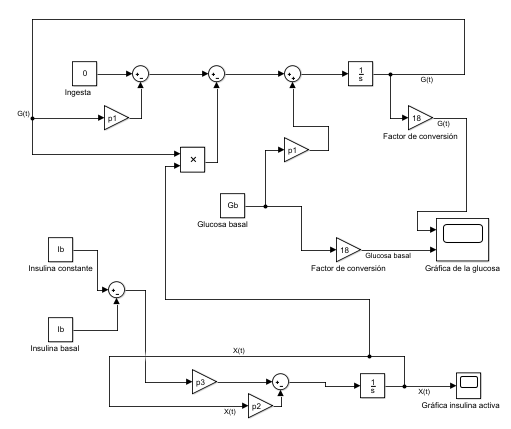
\includegraphics[width=0.9\linewidth]{img/anexos/bloques/modelo_bergman.png}
    \caption{Diagrama de bloques para el Modelo de Bergman.}
    \label{fig:diag_bergman}
\end{figure}

La equivalencia de la Figura \ref{fig:diag_bergman} a nivel matemático es:
\begin{align}
    \frac{dG(t)}{dt}= -p_1 (G(t) - G_b) - X(t)G(t) , G(0) = Gb
    \label{eq:ecBergGluc}\\
    \frac{dX(t)}{dt}= -p_2 X(t) + p_3(I(t) - I_b),    X(0) = 0
    \label{eq:ecBergInsAc}
\end{align}
\clearpage
Cuando no se trabaja con una insulina constante, se añade una tercera ecuación al sistema, que modela la insulina a lo largo del tiempo. También tiene caracter diferencial y permite aproximar a la realidad el comportamiento de la glucosa e insulina en el organismo. 
Se añade al sistema anterior formado por las ecuaciones (\ref{eq:ecBergGluc}) y (\ref{eq:ecBergInsAc}), la ecuación (\ref{eq:insulina_variable}), representada en la Figura \ref{fig:diag_ins_var}.

\begin{equation}
    \frac{dI(t)}{dt} = p_6 (G(t)-p_5)^+ t -n(I(t)+Ib), Ib(0)=0
    \label{eq:insulina_variable}
\end{equation}

\begin{figure}[htbp]
    \centering
    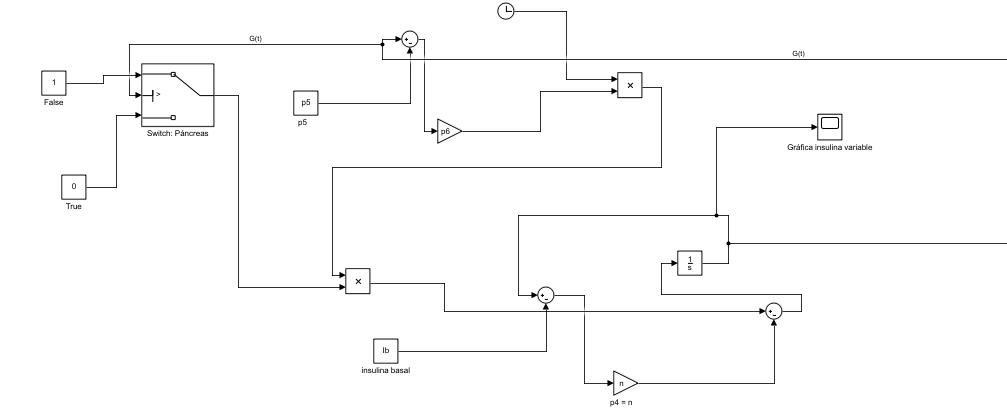
\includegraphics[width=1\linewidth]{img/anexos/bloques/ins_variable.png}
    \caption{Diagrama de bloques de la insulina variable en el Modelo de Bergman.}
    \label{fig:diag_ins_var}
\end{figure}

Se muestra en la Figura el Modelo de Bergman completo con la insulina I(t) variable modelada en la Figura \ref{fig:diag_ins_var}.
\clearpage

\begin{figure}[htbp]
    \centering
    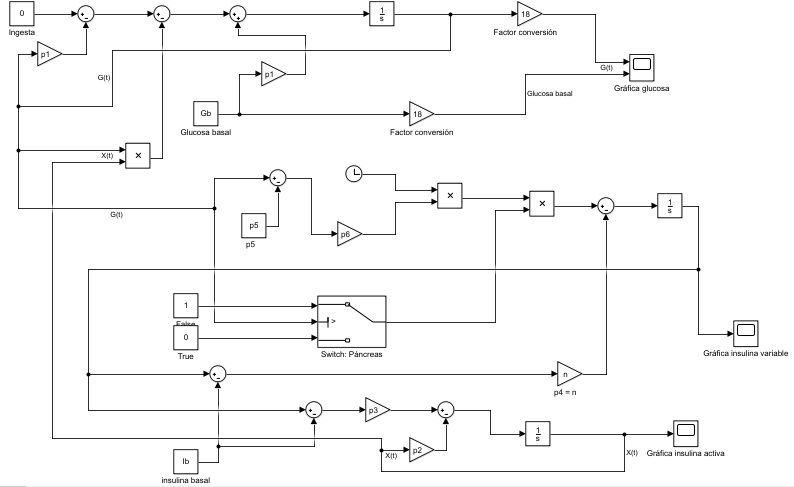
\includegraphics[width=1.2\linewidth]{img/anexos/bloques/insulina_var_completo.PNG}
    \caption{Diagrama de bloques del Modelo de Bergman con insulina variable.}
    \label{fig:diag_ins_var_completo}
\end{figure}
\clearpage
\subsection{Modelo Modificado}

Para el Modelo de Bergman Modificado, se lleva a cabo una variación en la ecuación de la insulina (\ref{eq:ecBergMod}) con el fin de incluir la variable insulina exógena U. 

De esta forma, el sistema resultante del Modelo Modificado es el siguiente:

\begin{align}
    \frac{dG(t)}{dt}= -p_1 (G(t) - G_b) - X(t)G(t), G(0)=Gb \\ \label{eq:glucosa_mod_mod}
    \frac{dX(t)}{dt}= -p_2 X(t) + p_3(I(t) - I_b), X(0) = 0 \\
    \frac{dI(t)}{dt}= -n I(t) + \frac{U(t)}{Vi}, I(0) = Ib 
    \label{eq:ecBergMod}
\end{align}

Se muestra en la Figura \ref{fig:diag_mod_bergman} el diagrama de bloques empleado.

\begin{figure}[htbp]
    \centering
    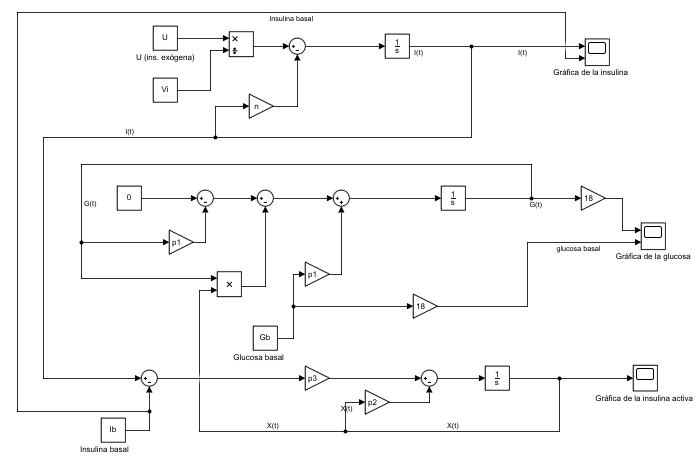
\includegraphics[width=1\linewidth]{img/anexos/completo_bergman_modificado.png}
    \caption{Diagrama de bloques para el Modelo Modificado de Bergman.}
    \label{fig:diag_mod_bergman}
\end{figure}
\clearpage
Se incluye a continuación la implementación de las funciones ingesta (Figura \ref{fig:diag_ingesta}) y ejercicio físico (Figura \ref{fig:diag_ejercicio}) para el Modelo Modificado de Bergman. Ambas se encuentran unidas a la entrada del sistema, que es el tiempo, representado mediante un bloque \textit{Clock}. Además, se introducen como bloques denominados \textit{MatLab Function}.

\begin{figure}[htbp]
    \centering
    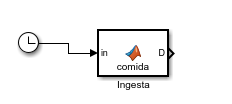
\includegraphics[width=0.5\linewidth]{img/anexos/bloques/ingesta.png}
    \caption{Inclusión de la ingesta en el Modelo Modificado.}
    \label{fig:diag_ingesta}
\end{figure}

\begin{figure}[htbp]
    \centering
    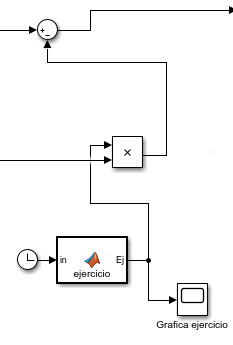
\includegraphics[width=0.4\linewidth]{img/anexos/bloques/ejercicio.png}
    \caption{Inclusión del ejercicio en el Modelo Modificado.}
    \label{fig:diag_ejercicio}
\end{figure}
Ambas variables y sus bloques incluidos en el Modelo Modificado se encuentran en la Figura \ref{fig:diag_completo_modificado}, así como el sistema de ecuaciones \ref{eq:ejercicio_ing_comp} formado.
\clearpage

\begin{align} 
    \frac{dG(t)}{dt}= -p_1 (G(t) - G_b) - X(t)Ej(t)G(t)+D(t), G(0)=Gb \\
    \frac{dX(t)}{dt}= -p_2 X(t) + p_3(I(t) - I_b), X(0) = 0 \\
    \frac{dI(t)}{dt}= -n I(t) + \frac{U(t)}{Vi}, I(0) = Ib \\
    \label{eq:ejercicio_ing_comp}
\end{align}

\begin{figure}[htbp]
    \centering
    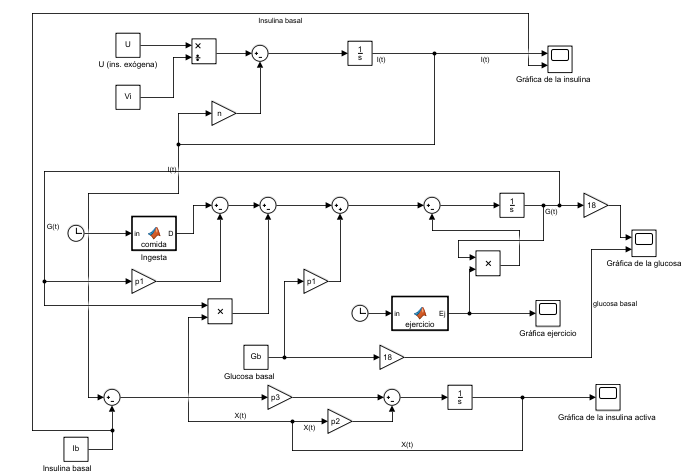
\includegraphics[width=1\linewidth]{img/anexos/bloques/mod_bergman_ej_ing.PNG}
    \caption{Diagrama de bloques del Modelo Modificado con el ejercicio físico y la ingesta.}
    \label{fig:diag_completo_modificado}
\end{figure}

\clearpage
El intento de modelización de la insulina rápida en el Modelo Modificado de Bergman se basa en el uso de un bloque \textit{Switch} conectado a una entrada (la glucosa G(t)), cuya salida puede ser True o False. Además, registra en su interior un umbral de glucosa, simulando el comportamiento del páncreas para el sistema.

\begin{figure}[htbp]
    \centering
    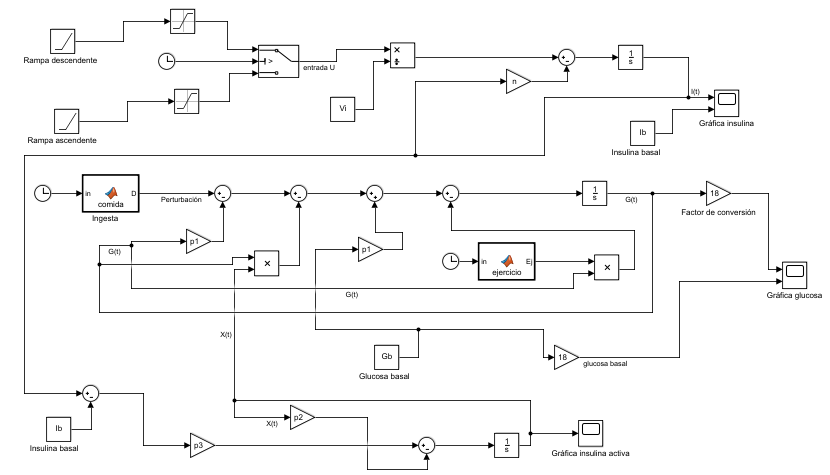
\includegraphics[width=1\linewidth]{img/anexos/bloques/completo_bergman_mod.PNG}
    \caption{Inclusión de la insulina rápida en el modelo.}
    \label{fig:diag_ins_rapida}
\end{figure}
\clearpage
\subsection{Regulación}

Respecto a este apartado, para introducir elementos regulatorios en Simulink basta con emplear el bloque \textit{PID Controller} y establecer los parámetros para los términos proporcional, integral y derivativo en su interior. Su salida se une a la entrada de la ecuación de la insulina, sustituyendo esta nueva unión por la insulina exógena que se administraba anteriormente.

Este implementación se puede observar en la Figura \ref{fig:diag_reg}.

\begin{figure}[htbp]
    \centering
    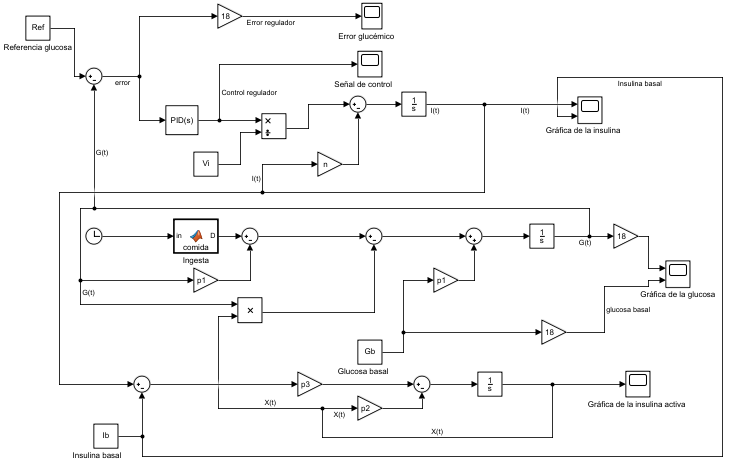
\includegraphics[width=1\linewidth]{img/anexos/bloques/regulacion_bueno.PNG}
    \caption{Inclusión de un regulador en el Modelo Modificado.}
    \label{fig:diag_reg}
\end{figure}

En función de las particularidades de cada regulador, se completan sus términos proporcional, integral y derivativo haciendo \textit{click} dentro del \textit{PID Controller}.

\clearpage

\section{Scripts}

Se incluyen a continuación los scrips ejecutados para llevar a cabo este análisis. Inicialmente, se encuentran los que inicializan las variables de un paciente no diabético (Figura \ref{fig:script_no_diab}), así como de un paciente diabético (Figura \ref{fig:script_diab}).

\begin{figure}[htbp]
    \centering
    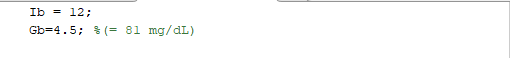
\includegraphics[width=0.8\linewidth]{img/anexos/codigo/no_Diabetico.PNG}
    \caption{Código para el establecimiento de los valores de un paciente no diabético.}
    \label{fig:script_no_diab}
\end{figure}
\begin{figure}[htbp]
    \centering
    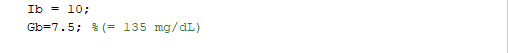
\includegraphics[width=0.8\linewidth]{img/anexos/codigo/diabetico.PNG}
    \caption{Código para el establecimiento de los valores de un paciente diabético.}
    \label{fig:script_diab}
\end{figure}


\subsection{Modelo de Bergman}

\subsubsection{Parámetros del Modelo}

El script necesario para inicializar los parámetros del Modelo se encuentra en la siguiente Figura \ref{fig:script_parametros}:

\begin{figure}[htbp]
    \centering
    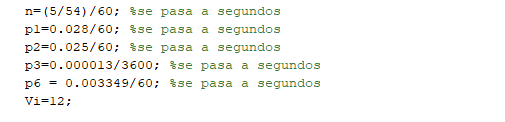
\includegraphics[width=0.8\linewidth]{img/anexos/codigo/p1_p2.PNG}
    \caption{Código para inicializar los parámetros del Modelo de Bergman.}
    \label{fig:script_parametros}
\end{figure}
\clearpage
El estudio de la variación de los parámetros p1, p2 y p3 se recoge en la siguiente Figura \ref{fig:script_var_param}:

\begin{figure}[htbp]
    \centering
    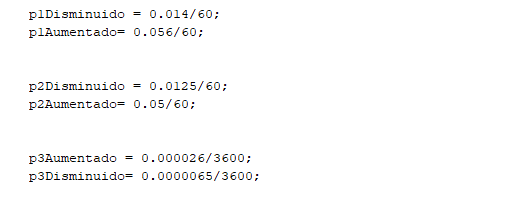
\includegraphics[width=0.8\linewidth]{img/anexos/codigo/variacion_param.PNG}
    \caption{Código para estudiar la variabilidad de los parámetros p1, p2 y p3 del Modelo de Bergman.}
    \label{fig:script_var_param}
\end{figure}


\subsection{Modelo Modificado}

A continuación, se detallan los scripts base correspondientes a las funciones ingesta y ejercicio físico (Figura \ref{fig:script_ingesta} y Figura \ref{fig:script_ejercicio}, respectivamente) , que se han visto modificados a lo largo de las secciones para realizar las distintas simulaciones. 

\begin{figure}[htbp]
    \centering
    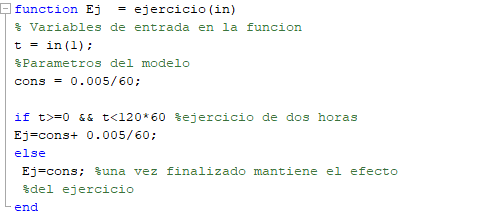
\includegraphics[width=0.8\linewidth]{img/anexos/codigo/funcion_ejercicio.png}
    \caption{Código de la función ejercicio para el Modelo Modificado.}
    \label{fig:script_ejercicio}
\end{figure}
\clearpage
\begin{figure}[htbp]
    \centering
    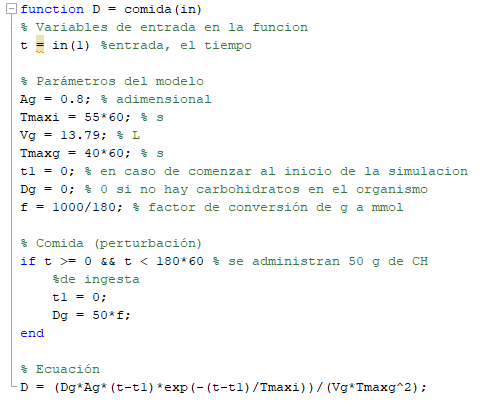
\includegraphics[width=0.8\linewidth]{img/anexos/codigo/funcion_ingesta.png}
    \caption{Código de la función ingesta para el Modelo Modificado.}
    \label{fig:script_ingesta}
\end{figure}

Por último para este apartado, para estudiar la variación de la constante de tiempo n se emplea el script de la Figura \ref{fig:script_n}:

\begin{figure}[htbp]
    \centering
    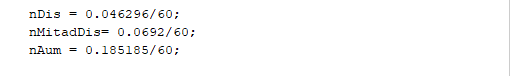
\includegraphics[width=0.8\linewidth]{img/anexos/codigo/variacion_n.PNG}
    \caption{Código para estudiar la variabilidad del parámetro n del Modelo de Bergman.}
    \label{fig:script_n}
\end{figure}


